The DEIMv2 training process was monitored for both site-specific datasets through TensorBoard, so as to track the evolution of validation accuracy and of the main loss terms across the 200 training epochs. These curves provide a compact view of the optimization dynamics and support the selection of the final checkpoint used for deployment.

In both experiments, the detector was trained for 200 epochs and the final model was selected according to the lowest validation loss observed during training. This criterion provided a consistent model-selection rule across the two datasets and made it possible to retain the checkpoint corresponding to the most favorable validation regime within the fixed training schedule.

\subsection{Site 1: Training on the Dough-Ball Dataset}
The first training experiment was carried out on the dough-ball dataset collected at Site~1 and composed by 50k images splitted 80, 10, 10. Figure~\ref{fig:DEIMv2_training_curves1} summarizes the main TensorBoard plots recorded during training. Overall, the curves indicate a stable optimization process, with progressive convergence of the loss terms and a validation trend that supports the selected final checkpoint.
%TODO: magari dividi le 4 figure in 2 e 2 perché se no va a capo nella pagina dopo con tutte e quattro e lascia un mega spazio bianco che non mi piace
\begin{figure}[h]
    \centering
    \begin{subfigure}[b]{0.48\textwidth}
        \centering
        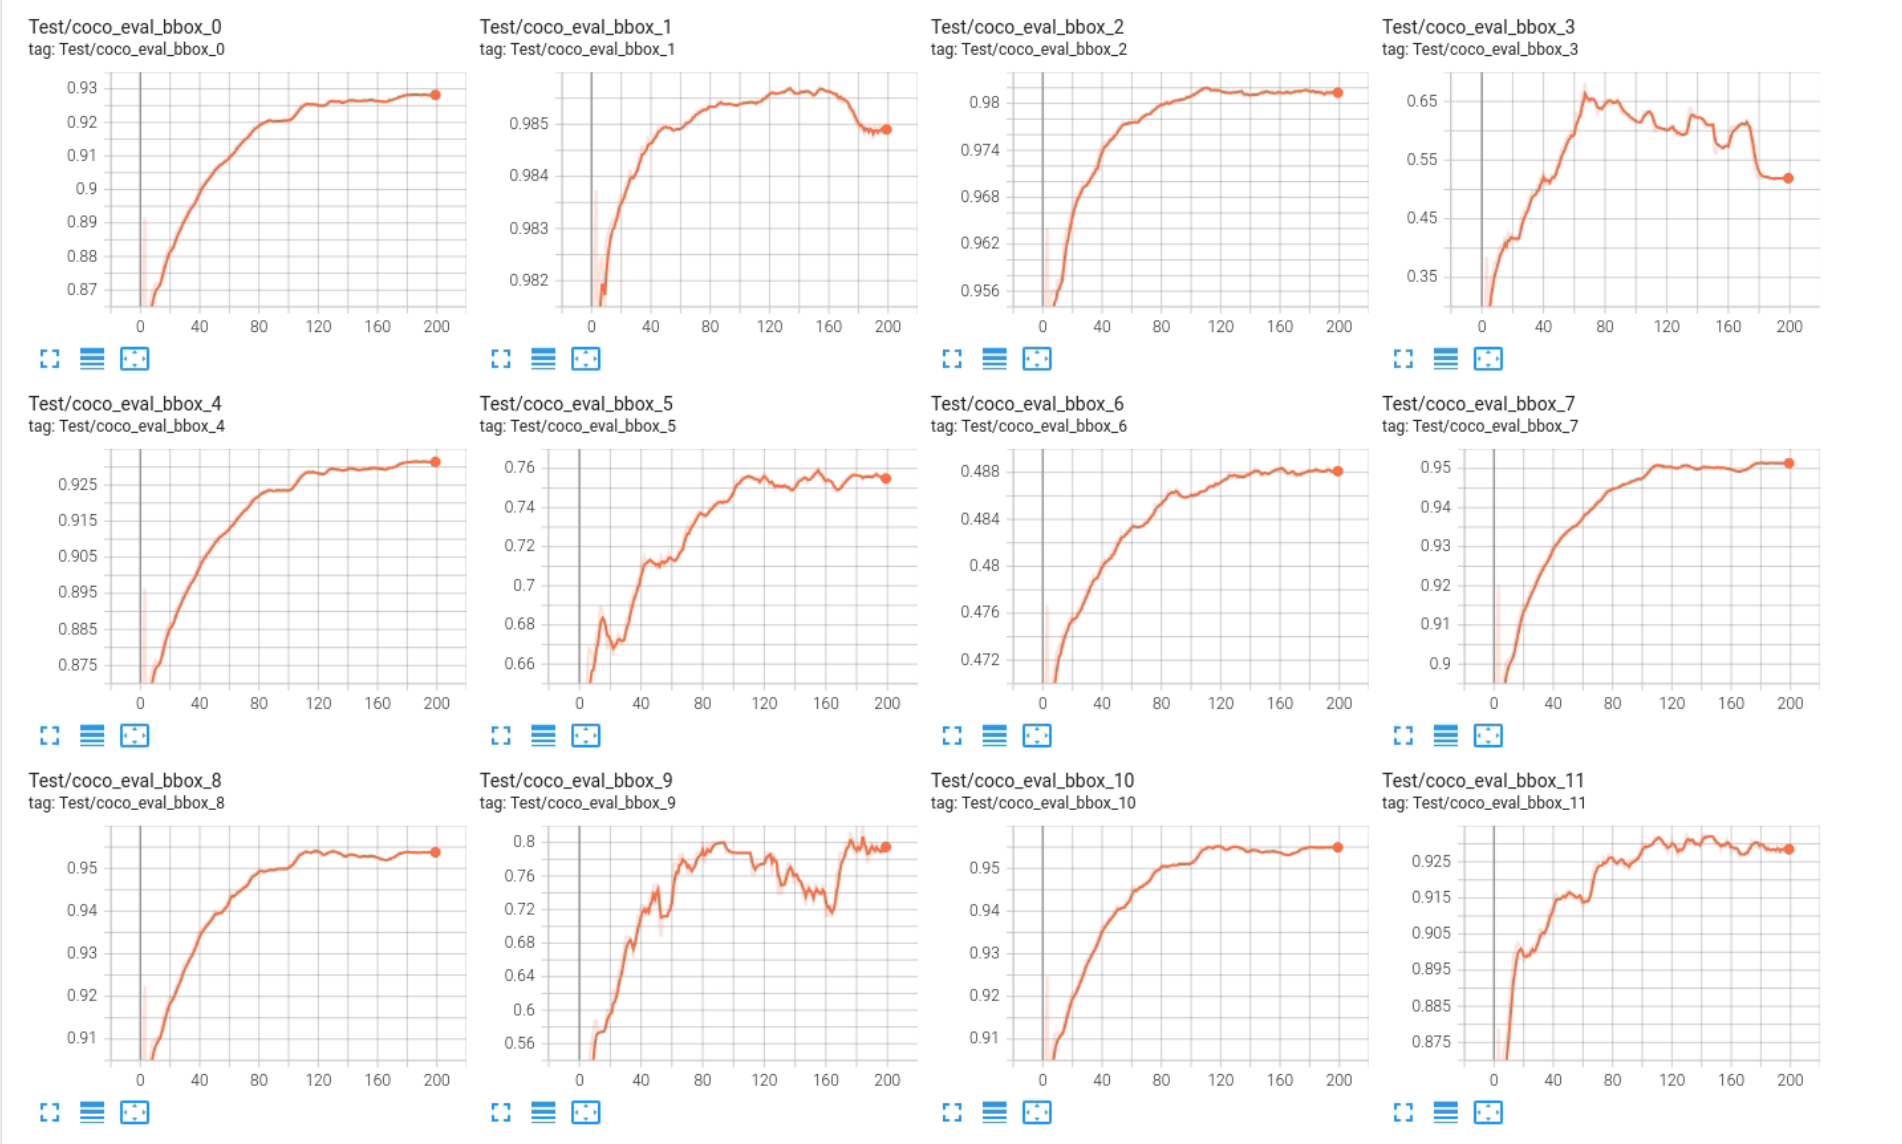
\includegraphics[width=\linewidth]{images/Tensor1_1.png}
        \caption{Validation accuracy}
    \end{subfigure}
    \hfill
    \begin{subfigure}[b]{0.48\textwidth}
        \centering
        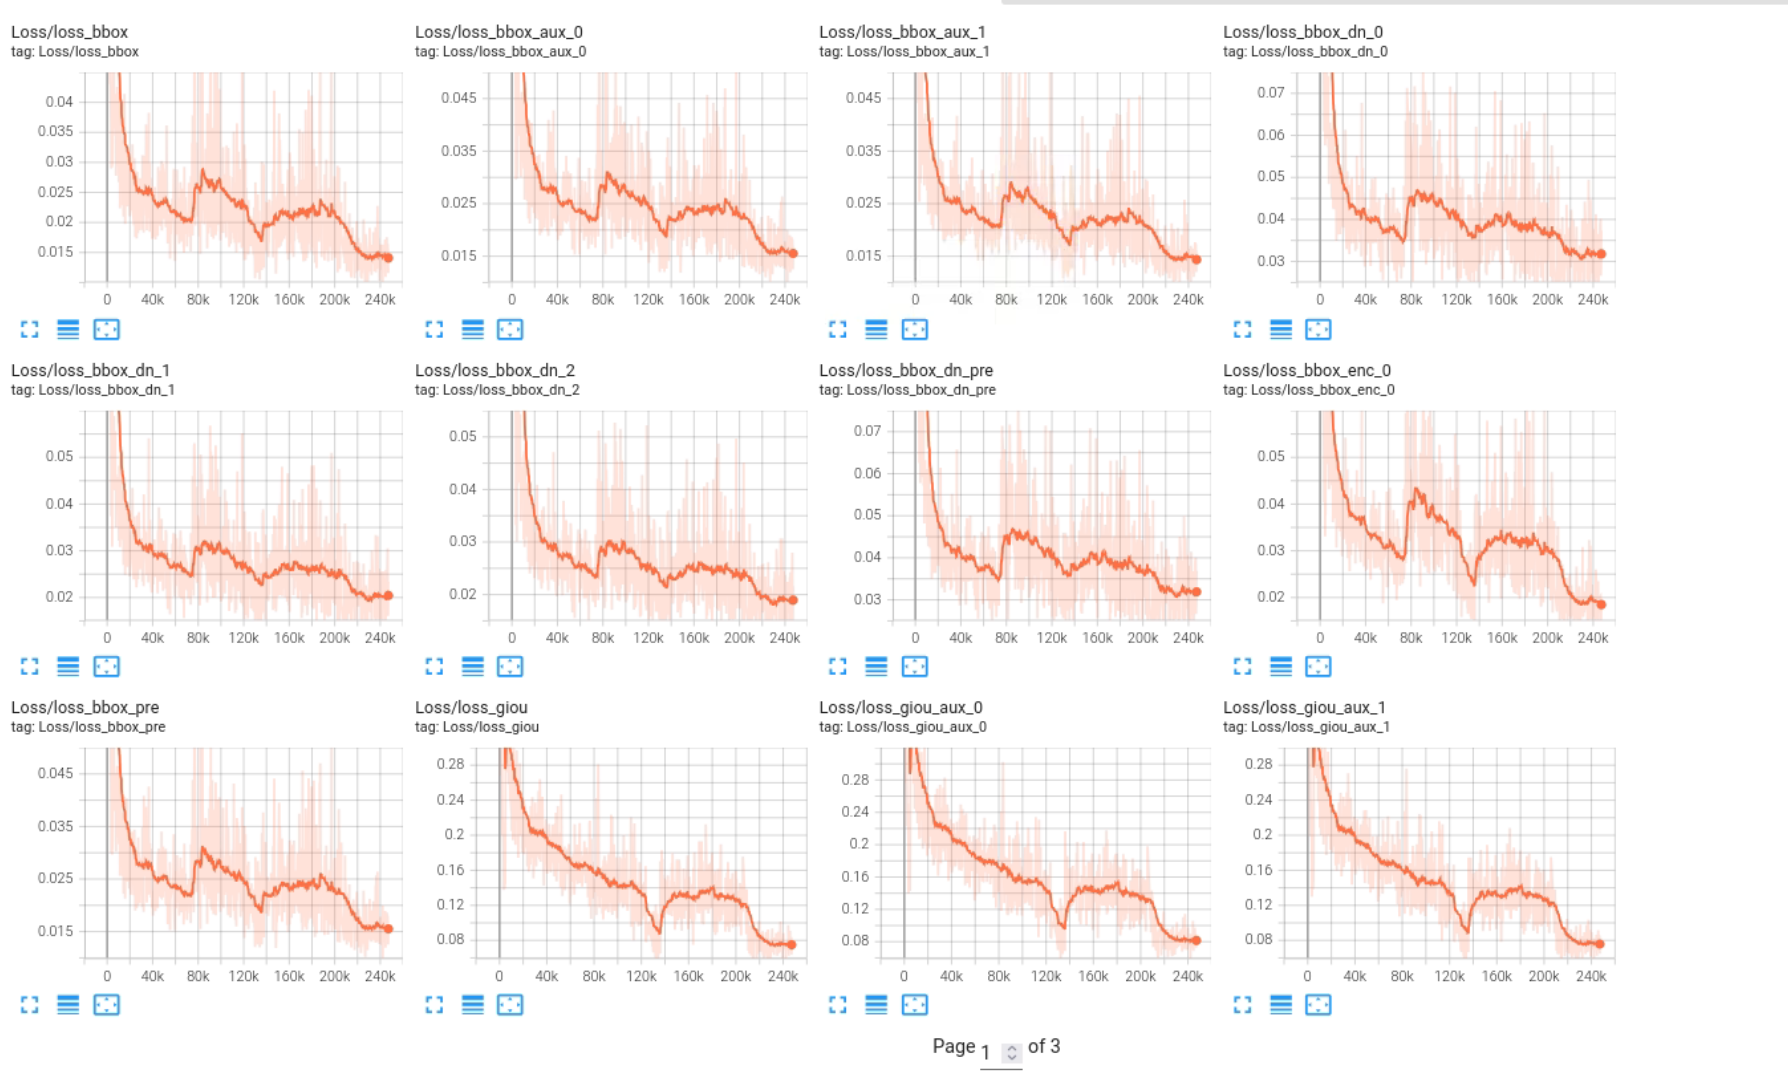
\includegraphics[width=\linewidth]{images/Tensor1_2.png}
        \caption{Loss term 1}
    \end{subfigure}

    \vspace{0.5em}

    \begin{subfigure}[b]{0.48\textwidth}
        \centering
        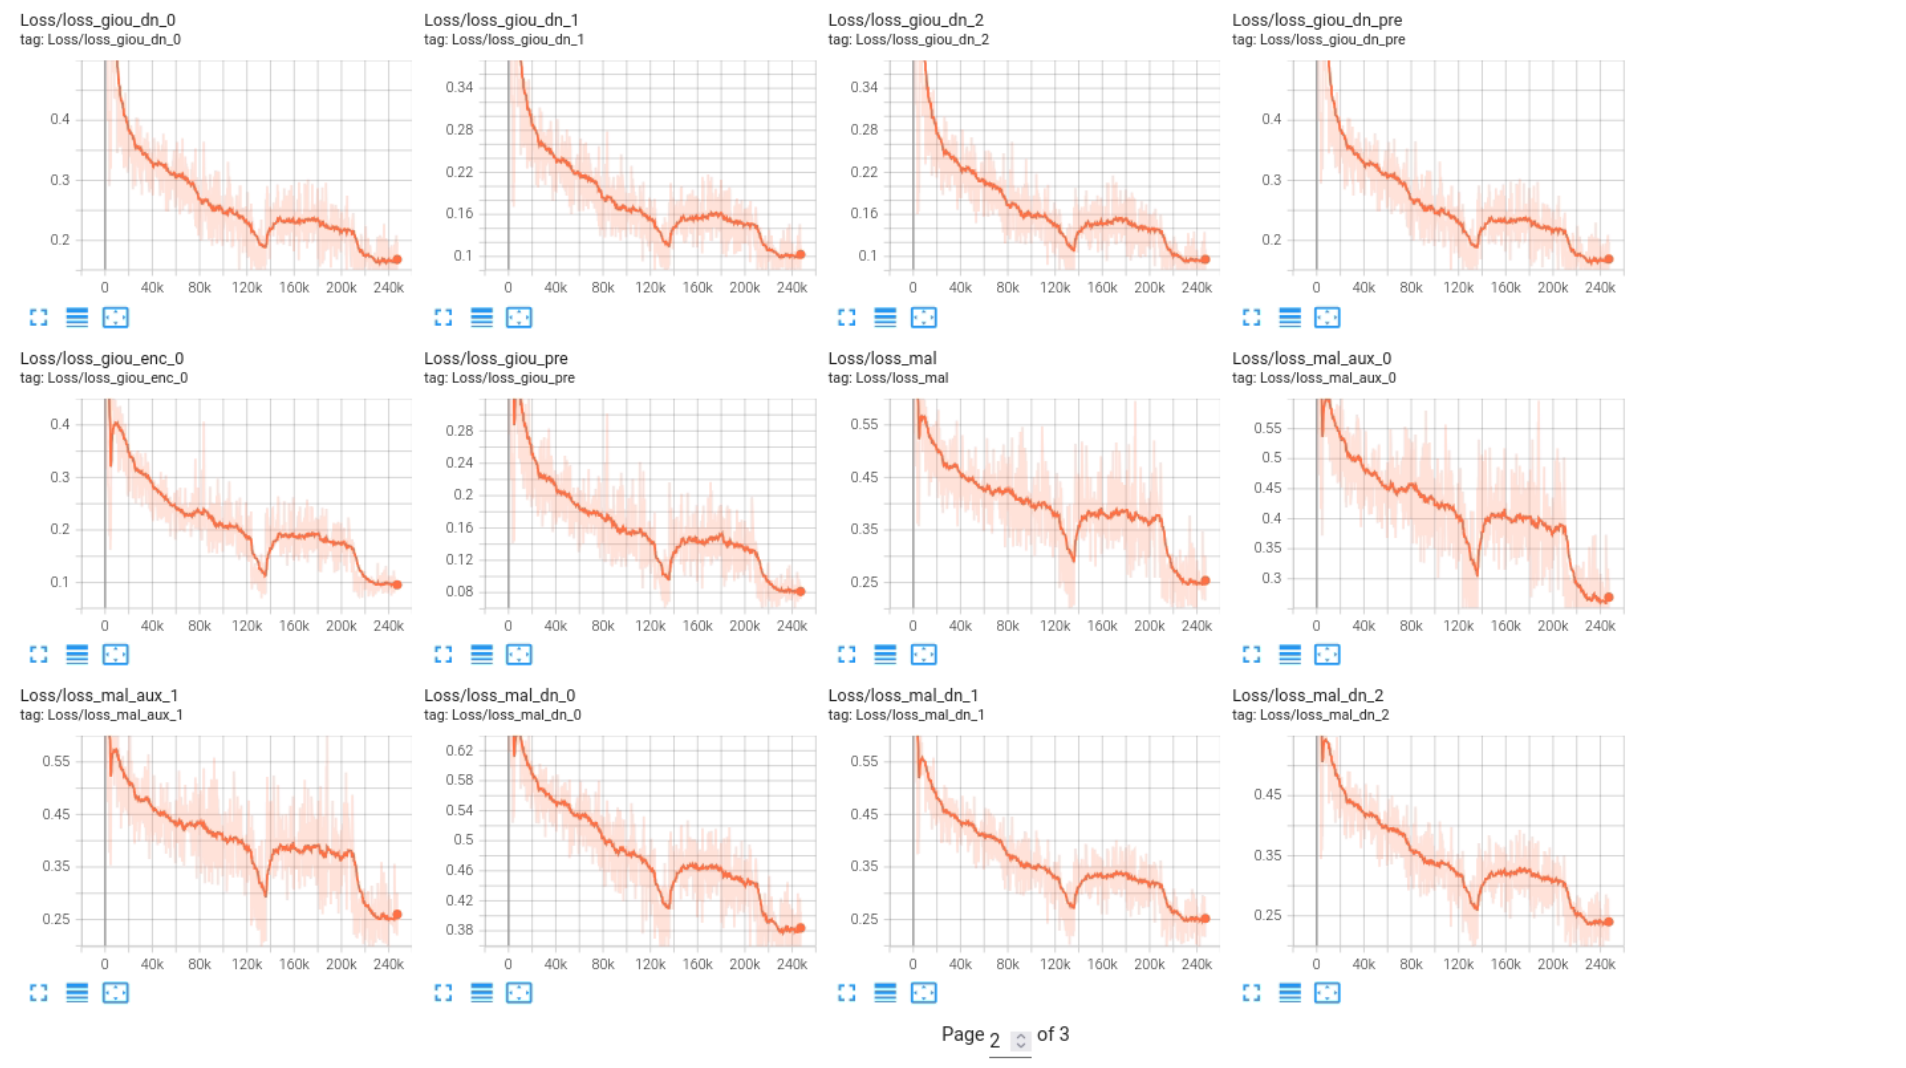
\includegraphics[width=\linewidth]{images/Tensor1_3.png}
        \caption{Loss term 2}
    \end{subfigure}
    \hfill
    \begin{subfigure}[b]{0.48\textwidth}
        \centering
        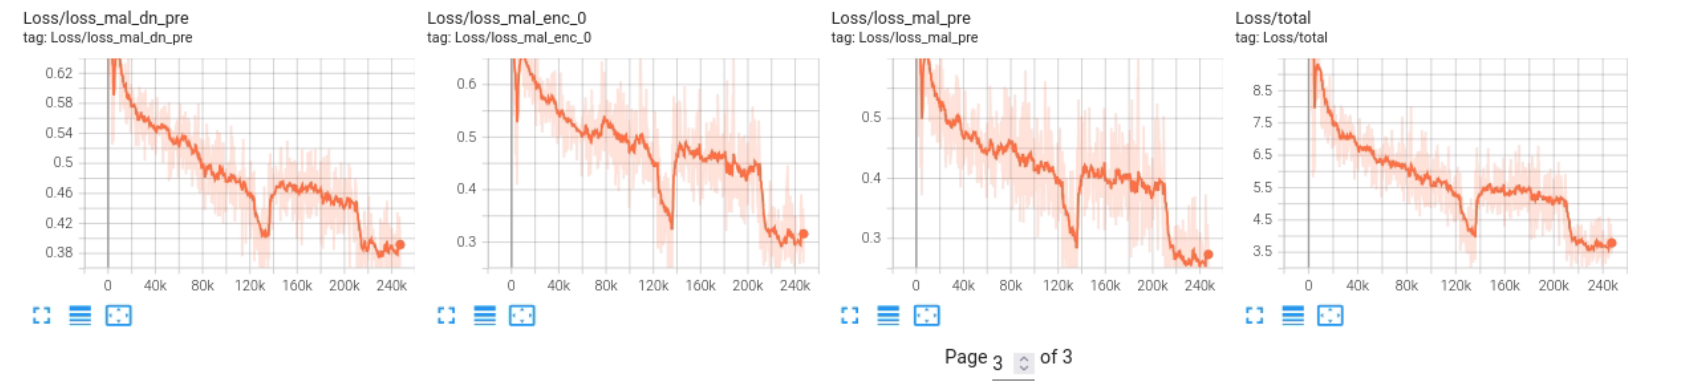
\includegraphics[width=\linewidth]{images/Tensor1_4.png}
        \caption{Loss term 3}
    \end{subfigure}
    \caption{TensorBoard monitoring of the DEIMv2 training on the Site~1 dough-ball dataset. The plots report the evolution of validation accuracy and of the main loss terms over the 200-epoch training schedule.}
    \label{fig:DEIMv2_training_curves1}
\end{figure}

The final detector achieved an Average Precision (AP) of 0.929 and an Average Recall (AR) of 0.953 on the evaluation split, indicating that the model was able to localize dough balls with high reliability despite the challenging visual configuration of the site.%TODO: come challenging con i dough balls che si toccano e si sovrappongono, magari aggiungi una frase del genere per spiegare meglio la difficoltà del dataset e giustificare il risultato leggermente inferiore rispetto a Site~2

\begin{figure}[h]
    \centering
    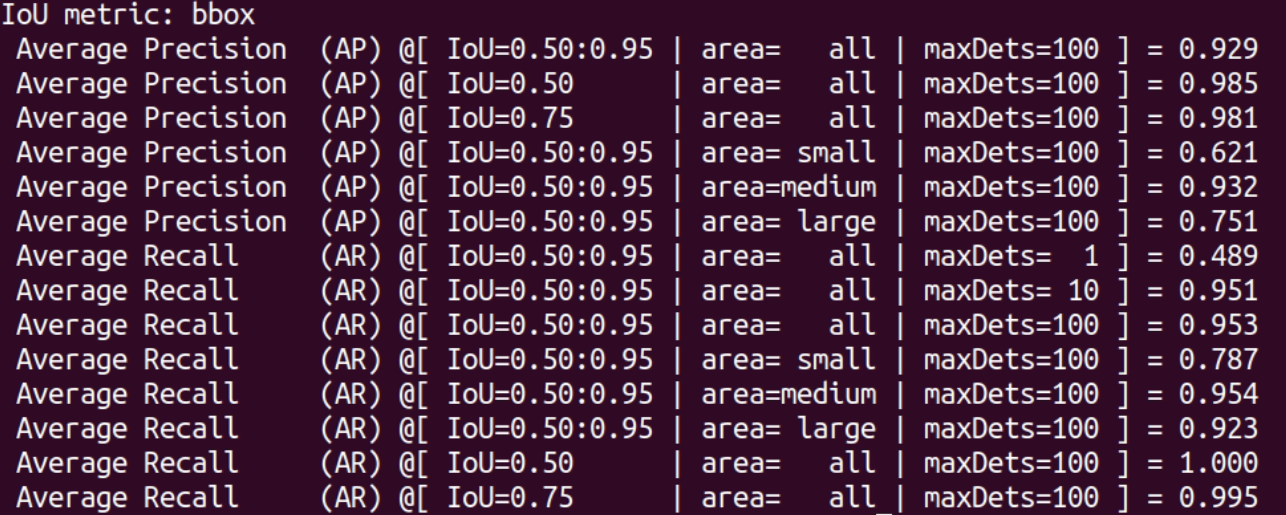
\includegraphics[width=0.7\textwidth]{images/DEIMv2_Results1.png}
    \caption{Quantitative DEIMv2 detection results obtained on the Site~1 dough-ball dataset.}
    \label{fig:DEIMv2_training_results1}
\end{figure}
\clearpage
\subsection{Site 2: Training on the Bread-Loaf Dataset}
The second training experiment was carried out on the bread-loaf dataset collected at Site~2, which consisted of 70k images, splitted 80, 10, 10. Also in this case, the TensorBoard plots in Figure~\ref{fig:DEIMv2_training_curves2} show a stable optimization process and support the checkpoint selected through the validation-loss criterion.

\begin{figure}[h]
    \centering
    \begin{subfigure}[b]{0.48\textwidth}
        \centering
        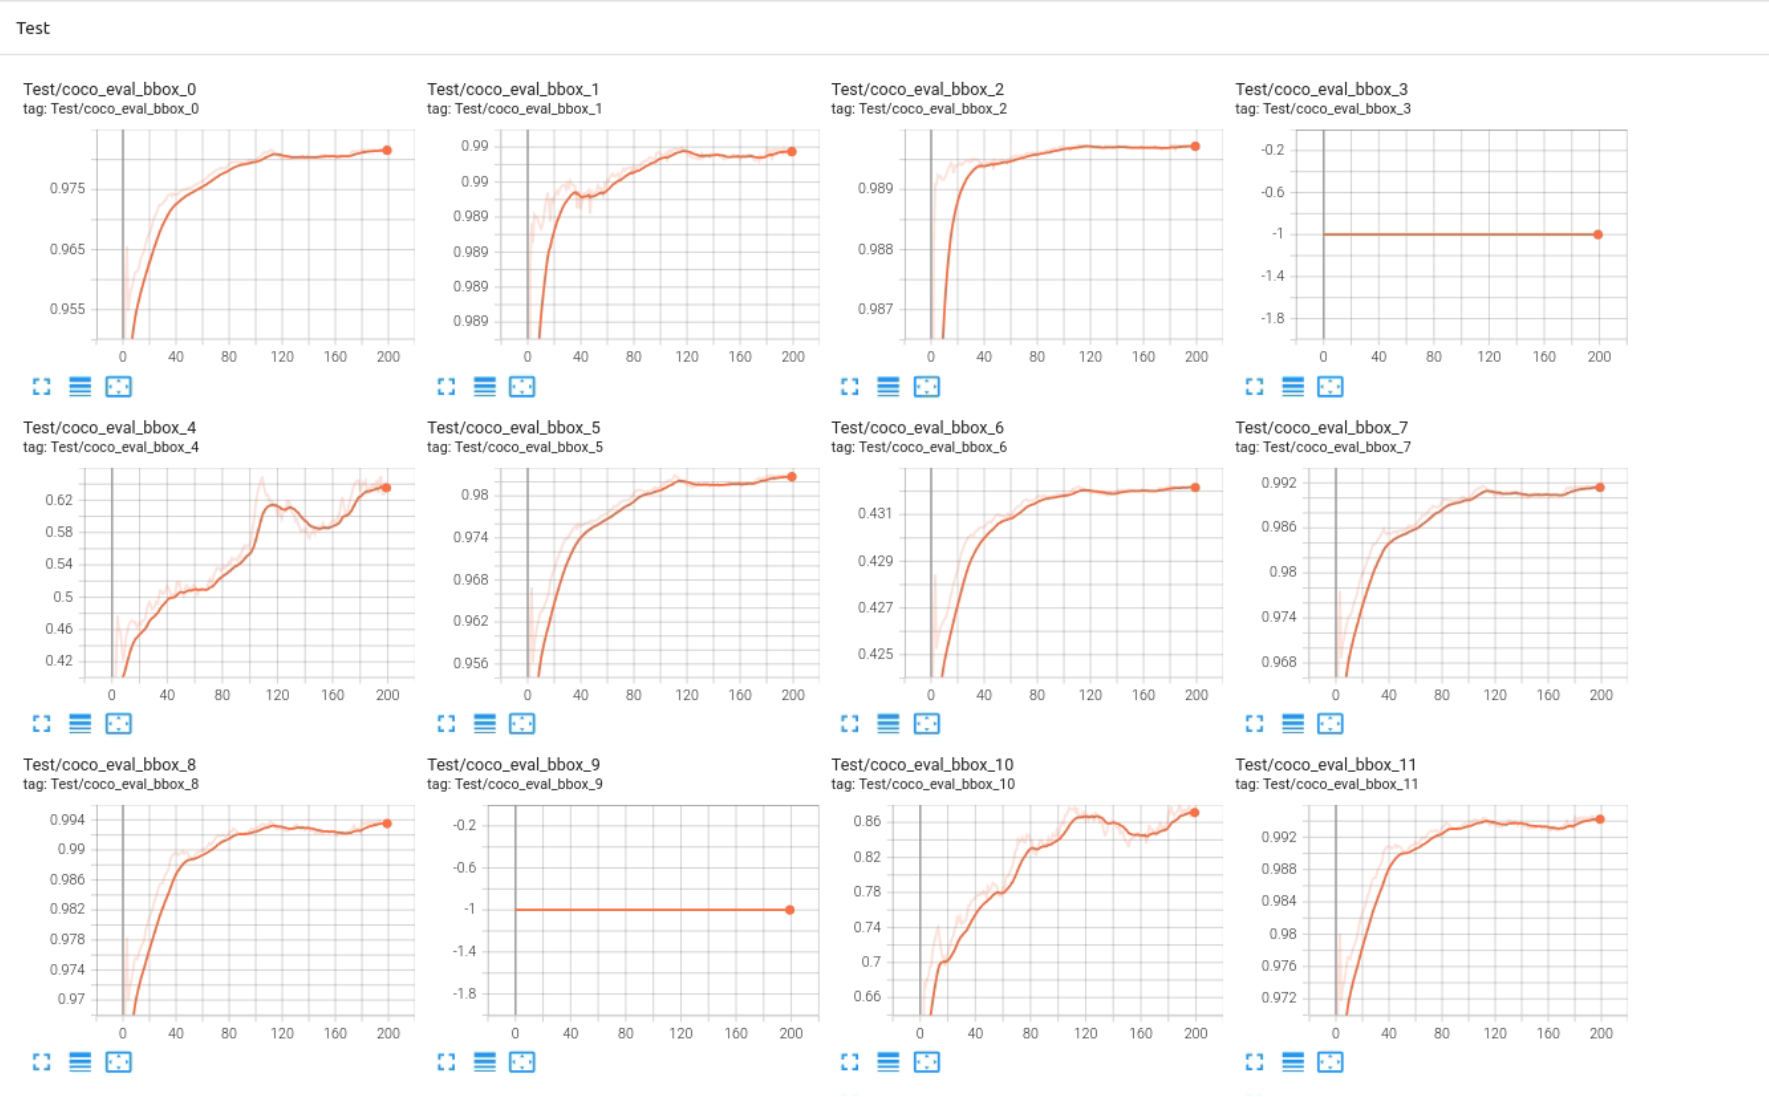
\includegraphics[width=\linewidth]{images/Tensor2_1.png}
        \caption{Validation accuracy}
    \end{subfigure}
    \hfill
    \begin{subfigure}[b]{0.48\textwidth}
        \centering
        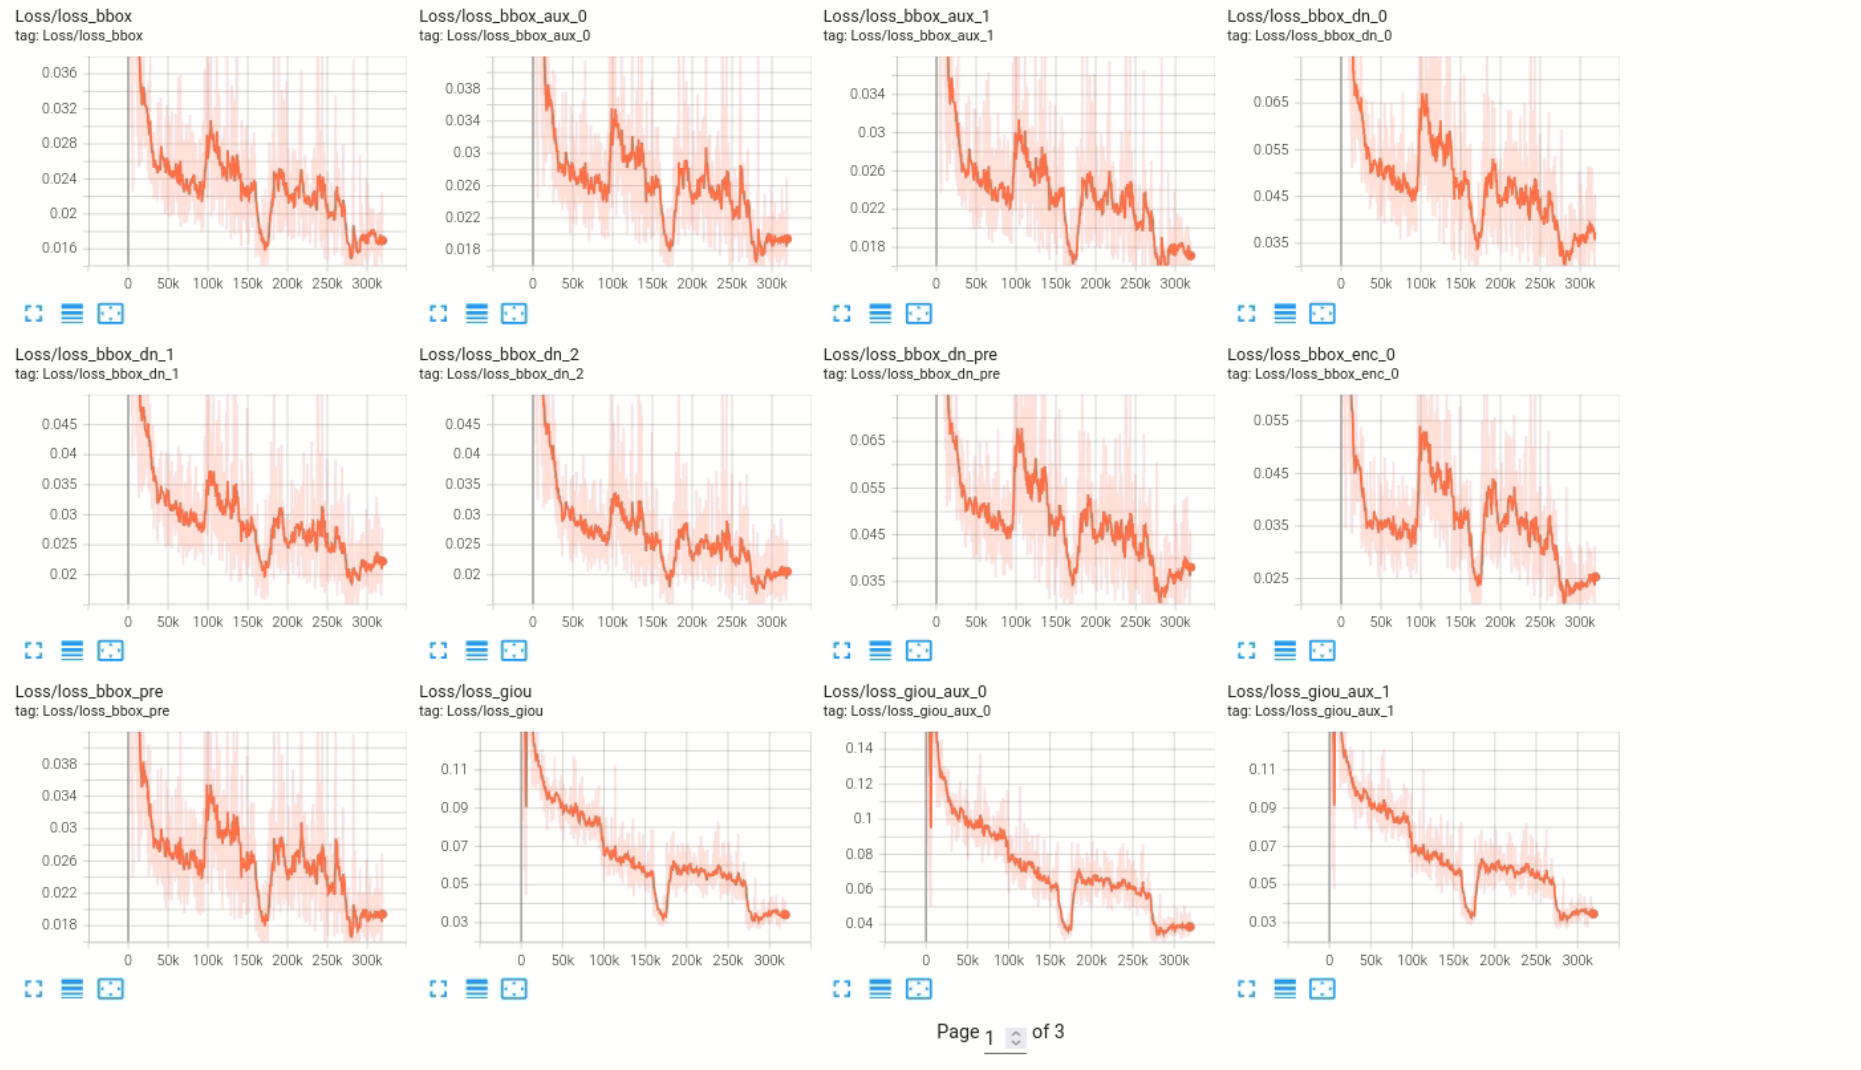
\includegraphics[width=\linewidth]{images/Tensor2_2.png}
        \caption{Loss term 1}
    \end{subfigure}

    \vspace{0.5em}

    \begin{subfigure}[b]{0.48\textwidth}
        \centering
        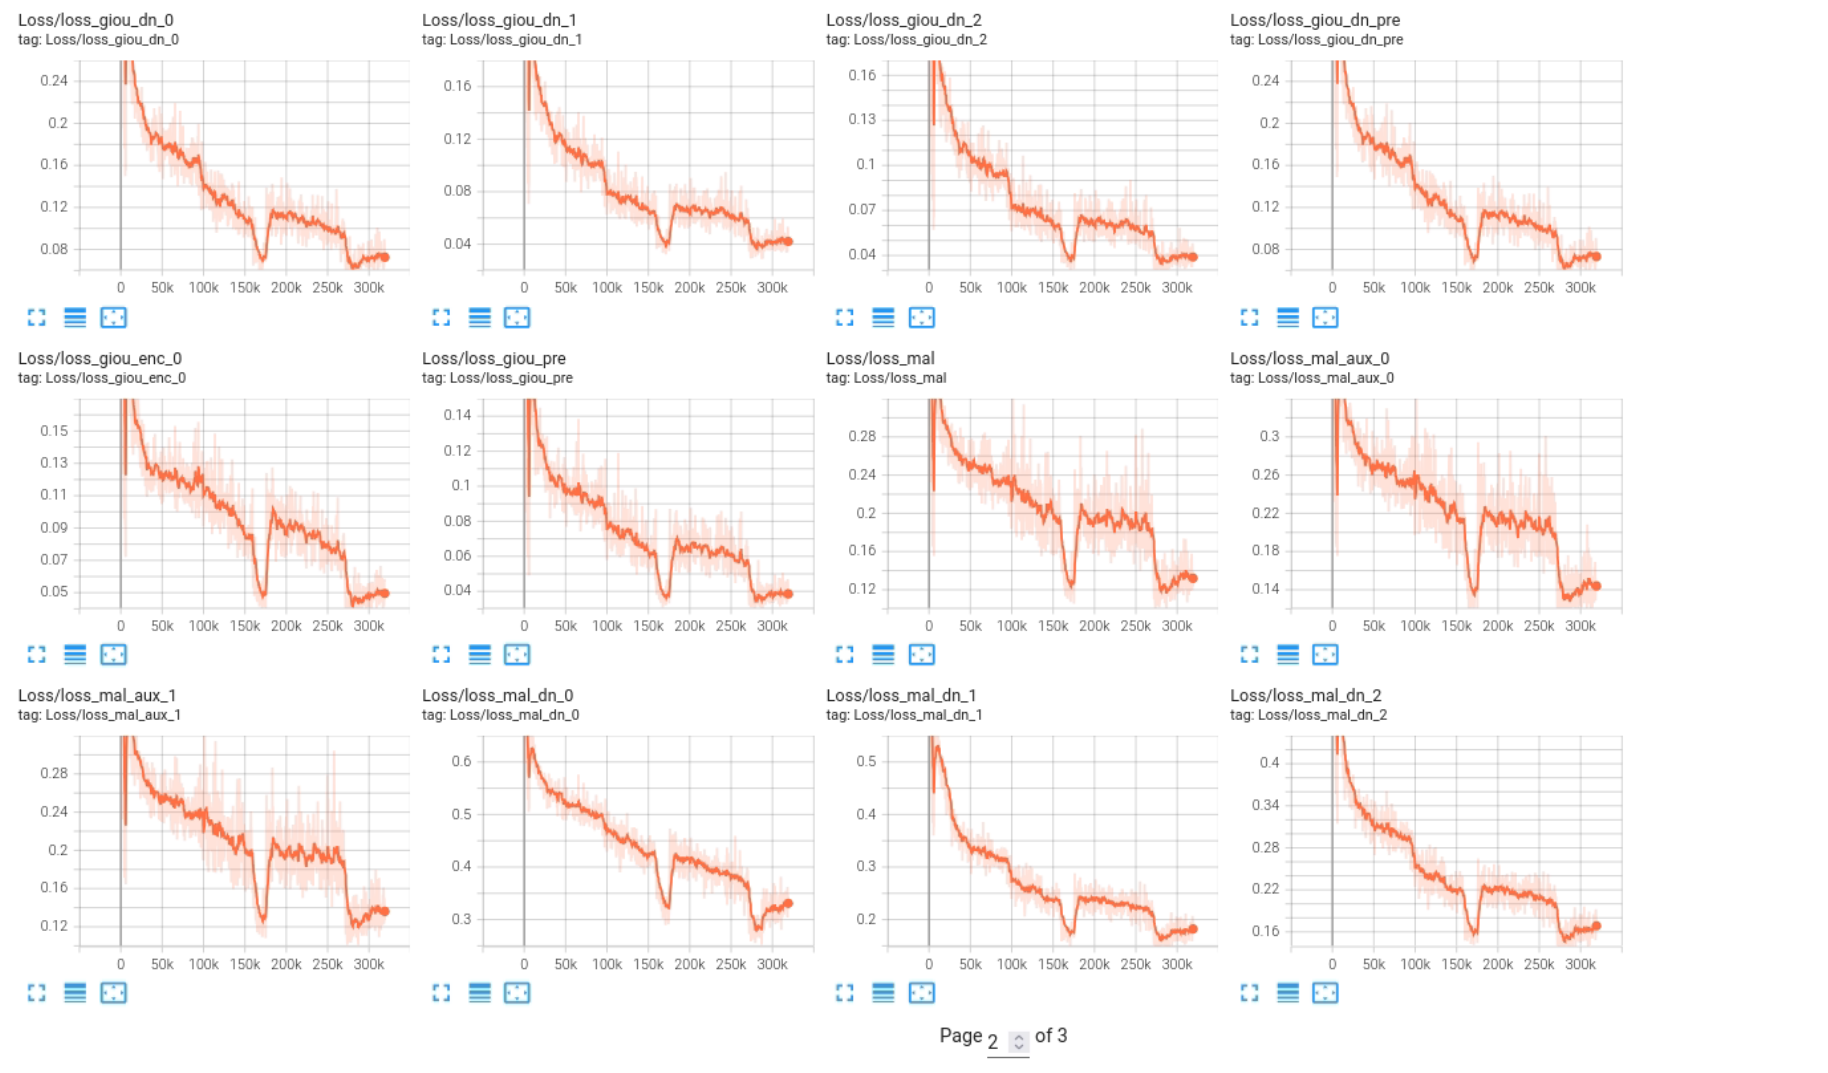
\includegraphics[width=\linewidth]{images/Tensor2_3.png}
        \caption{Loss term 2}
    \end{subfigure}
    \hfill
    \begin{subfigure}[b]{0.48\textwidth}
        \centering
        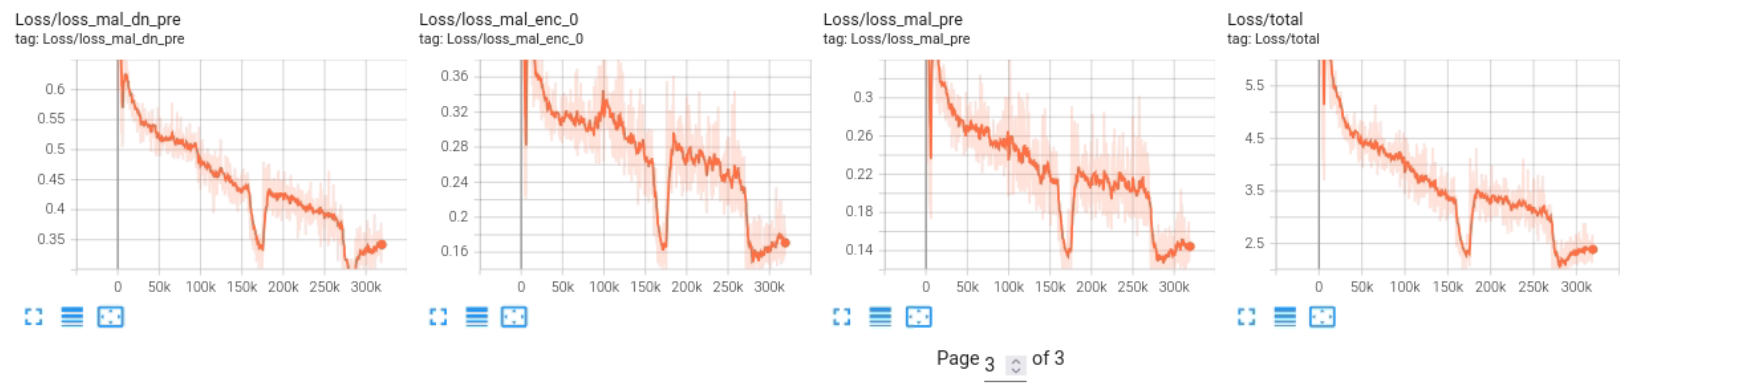
\includegraphics[width=\linewidth]{images/Tensor2_4.png}
        \caption{Loss term 3}
    \end{subfigure}
    \caption{TensorBoard monitoring of the DEIMv2 training on the Site~2 bread-loaf dataset. The plots report the evolution of validation accuracy and of the main loss terms over the 200-epoch training schedule.}
    \label{fig:DEIMv2_training_curves2}
\end{figure}

The final detector achieved an outstanding Average Precision (AP) of 0.982 and an Average Recall (AR) of 0.994 on the evaluation split, confirming that the model was able to localize bread loaves very accurately in the Site~2 setting.

\begin{figure}[h]
    \centering
    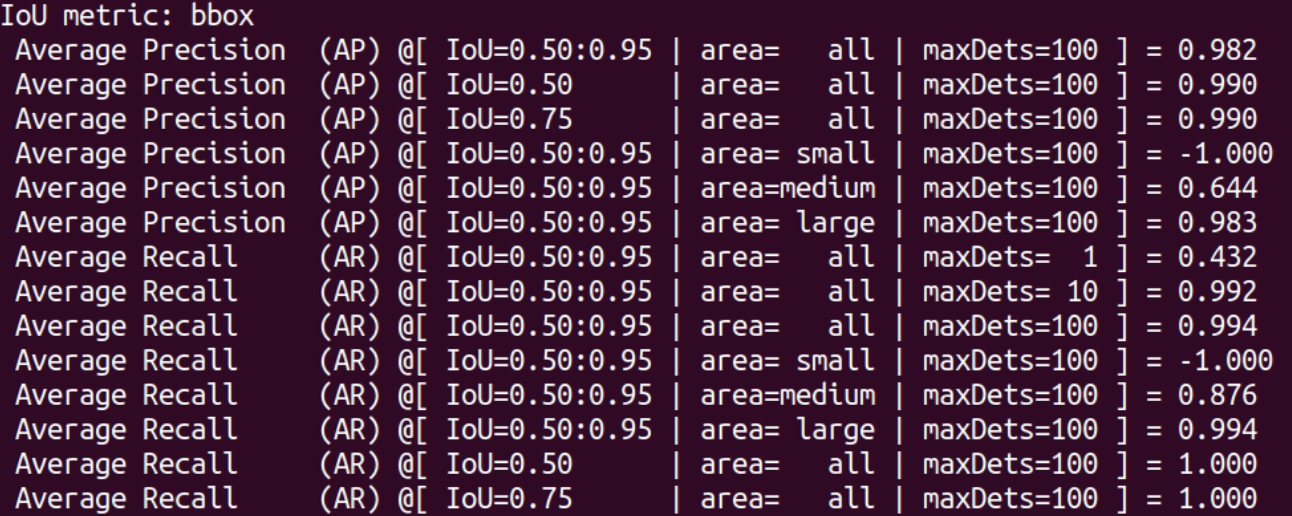
\includegraphics[width=0.7\textwidth]{images/DEIMv2_Results2.png}
    \caption{Quantitative DEIMv2 detection results obtained on the Site~2 bread-loaf dataset.}
    \label{fig:DEIMv2_training_results2}
\end{figure}

Comparing the two experiments, Site~2 achieved slightly higher detection performance than Site~1. A plausible explanation is the different visual complexity of the two datasets: at Site~1, dough balls may touch or partially overlap during production, making instance separation more difficult, whereas at Site~2 the bread loaves are generally more isolated and easier to localize. Since the same detector architecture and the same general training logic were used in both cases, this difference is likely associated more with dataset difficulty than with changes in the training procedure itself.
